\section{Gravity waves}

Gravity waves test taken from Weller and Shahrokhi.

\begin{itemize}
\item Reproduced result for BTF from W\&S
\item Vertical mixing at ground in lee of orography seen in results for snapCol and snap meshes.  This occurs in the lowest two rows of the mesh: lower layer $\theta$ is warmer, next layer above is cooler.  Feature is visible after t=3600s (Figure~\ref{fig:gw:mixing-3600s}), becomes more pronounced by t=18000s (Figure~\ref{fig:gw:mixing-18000s}).
\end{itemize}

\subsection{Investigation of vertical mixing}
Initially suspected mixing was due to computation mode of Lorenz vertical staggering but now it seems not:
\begin{itemize}
	\item plot UfDiff as a vector field doesn't seem to show any velocity anomalies in BTF or snalCol (Figure~\ref{fig:gw:ufdiff})
	\item plot of $\theta$ field shows that mixing is not strong enough to overcome stratification (Figure~\ref{fig:gw:theta})
	\item doubling mountain height causes mixing to appear in BTF case, and increases to three rows of mixing in SnapCol (Figure~\ref{fig:gw:double-height})
	\item halving $\Delta z$ also causes BTF mixing but less severe, also three rows of mixing in SnapCol (not shown)
	\item the results for dp/dx show mixing in BTF, and increased mixing in SnapCol (not shown)
\end{itemize}

\begin{figure}
	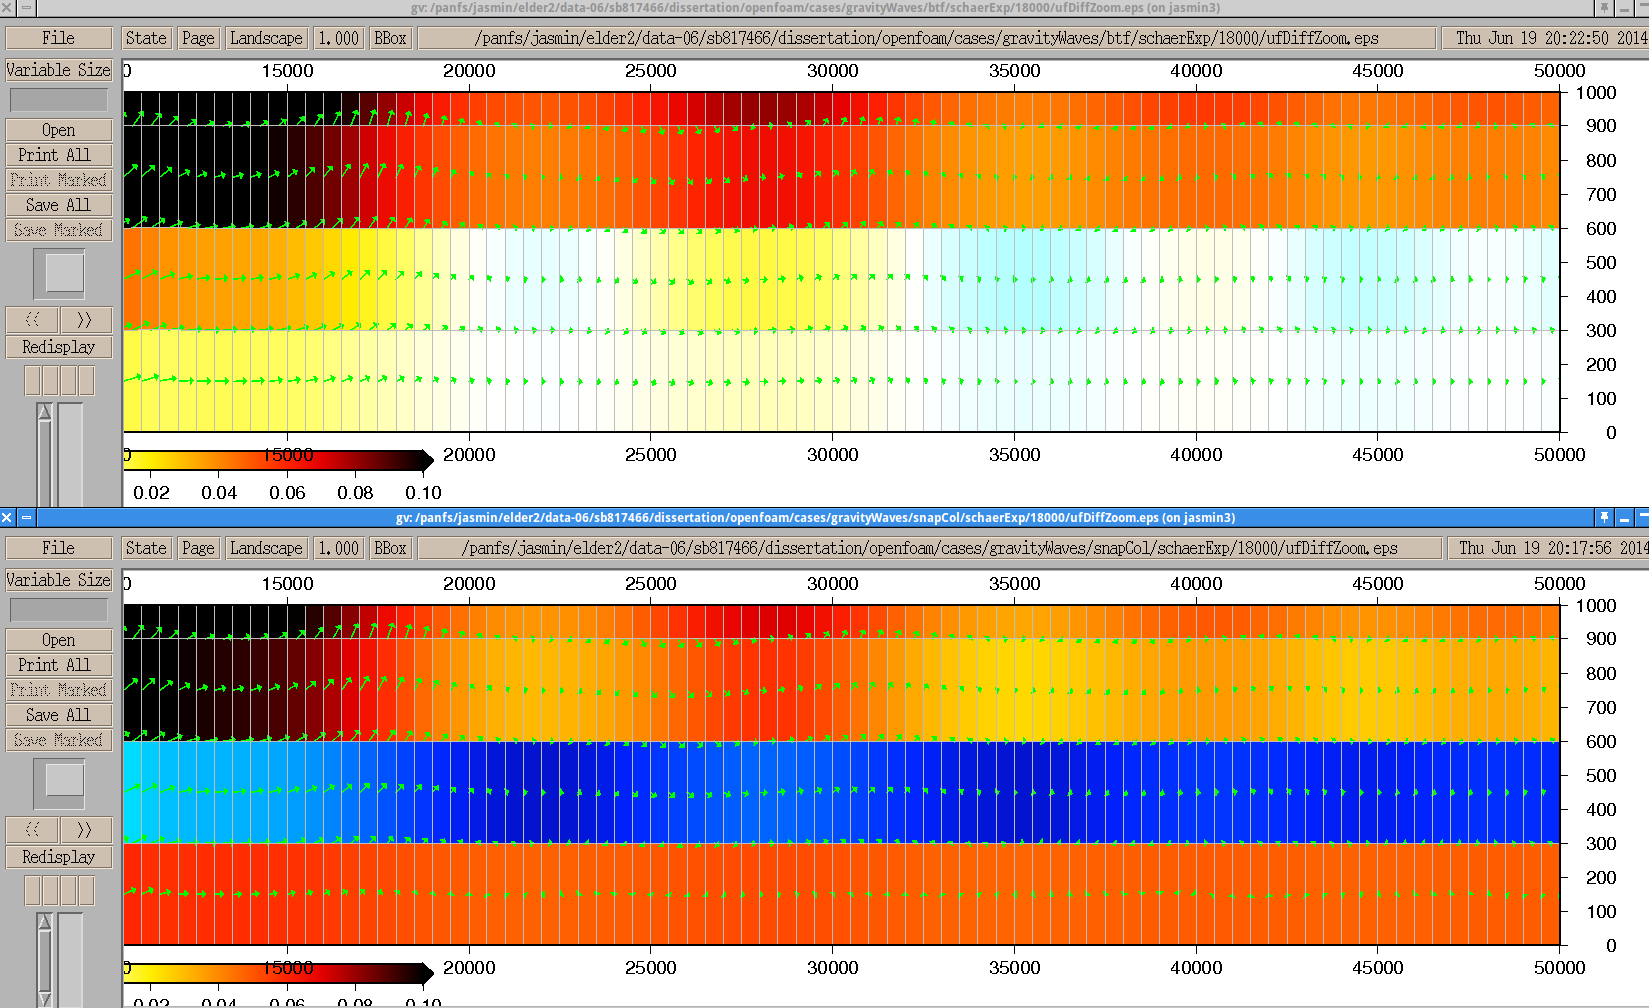
\includegraphics[width=\textwidth]{interim-results/gravityWavesBTFSnapColVelocityVectors.png}
	\caption{UfDiff after t=18000s, BTF and SnapCol meshes}
	\label{fig:gw:ufdiff}
\end{figure}

\begin{figure}
	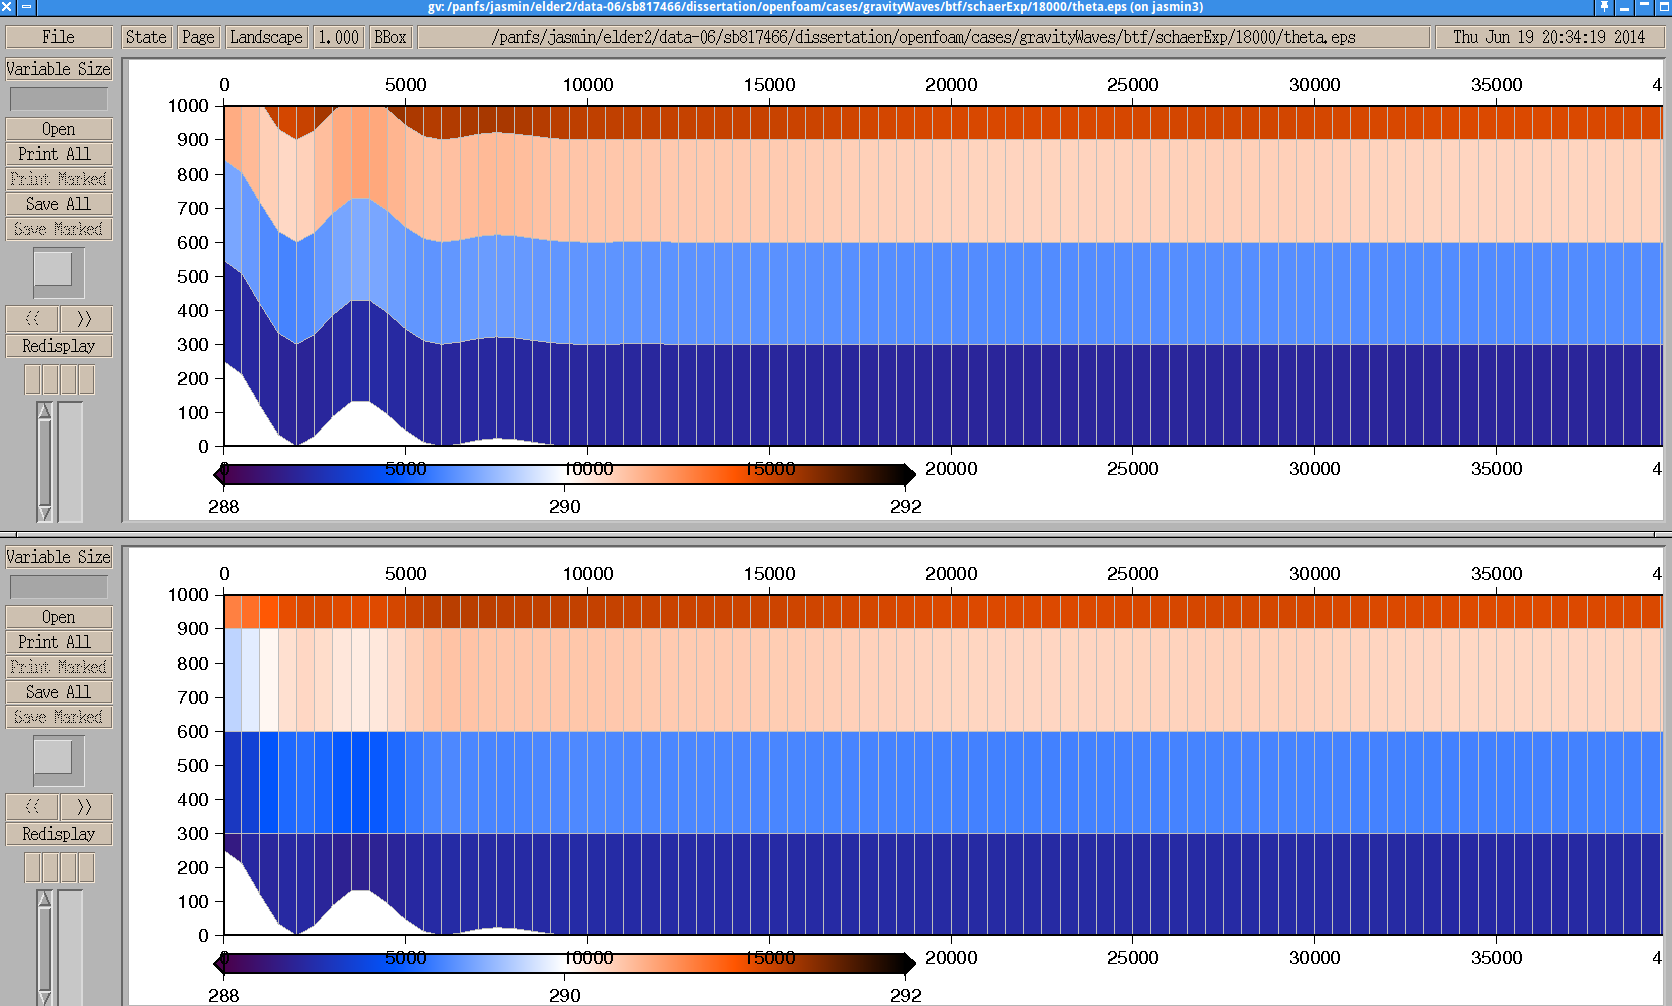
\includegraphics[width=\textwidth]{interim-results/gravityWavesBTFSnapColTheta.png}
	\caption{$\theta$ after t=18000s, BTF and SnapCol meshes}
	\label{fig:gw:theta}
\end{figure}

\begin{figure}
	BTF
	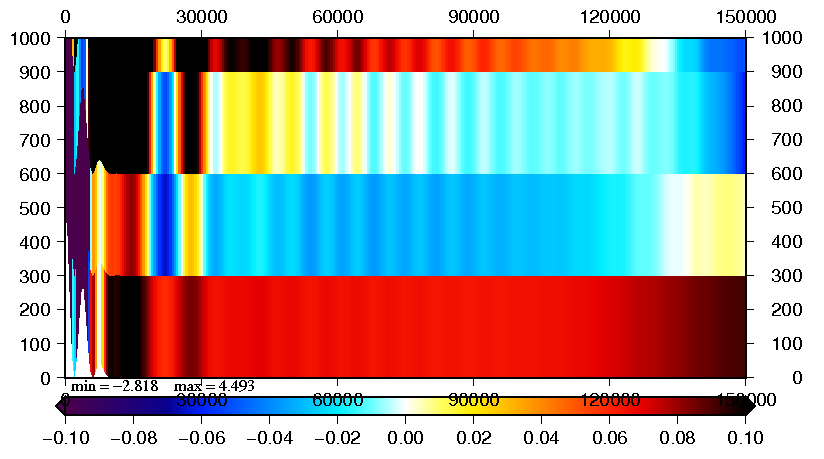
\includegraphics[width=\textwidth]{interim-results/gravityWavesBTFDoubleHeightThetaDiffZoom.png}
	SnapCol
	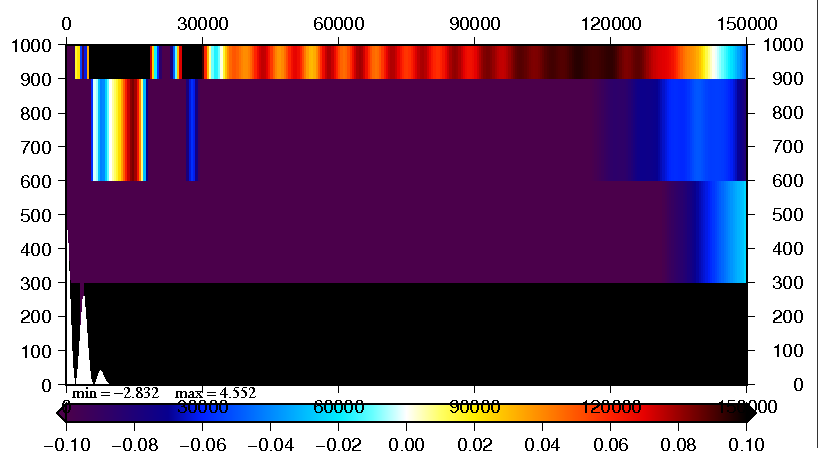
\includegraphics[width=\textwidth]{interim-results/gravityWavesSnapColDoubleHeightThetaDiffZoom.png}

	\caption{double height mountain, thetaDiff after t=18000s}
	\label{fig:gw:double-height}
\end{figure}

\begin{figure}
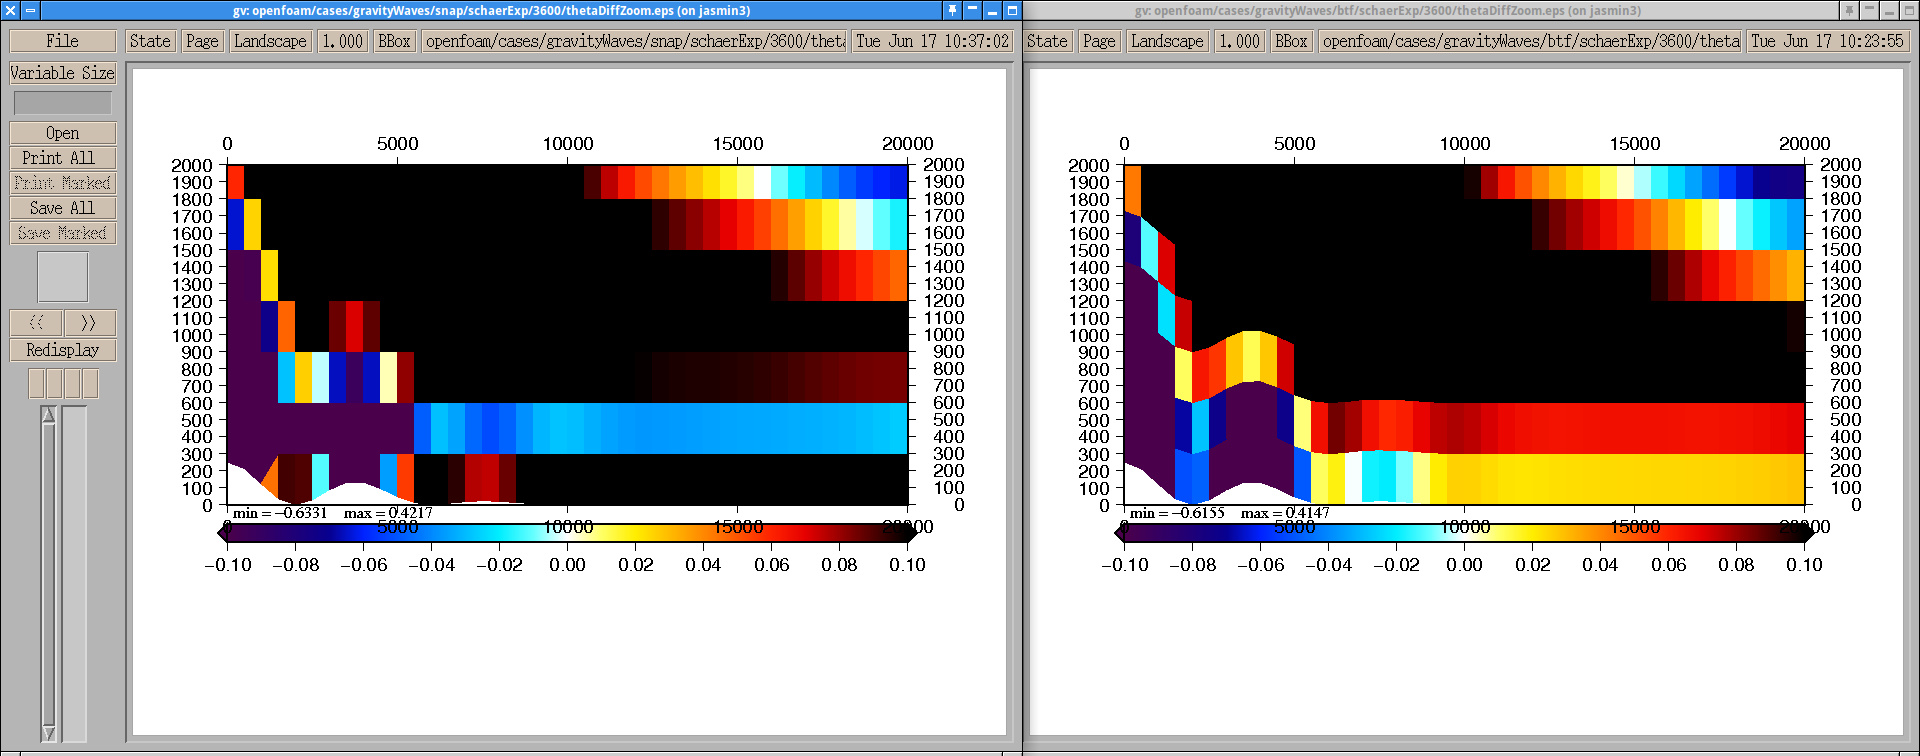
\includegraphics[width=\textwidth]{interim-results/gravityWavesBTFsnapMidZoom3600.png}
\caption{Vertical mixing after t=3600s, snap mesh left, BTF right}
\label{fig:gw:mixing-3600s}
\end{figure}

\begin{figure}
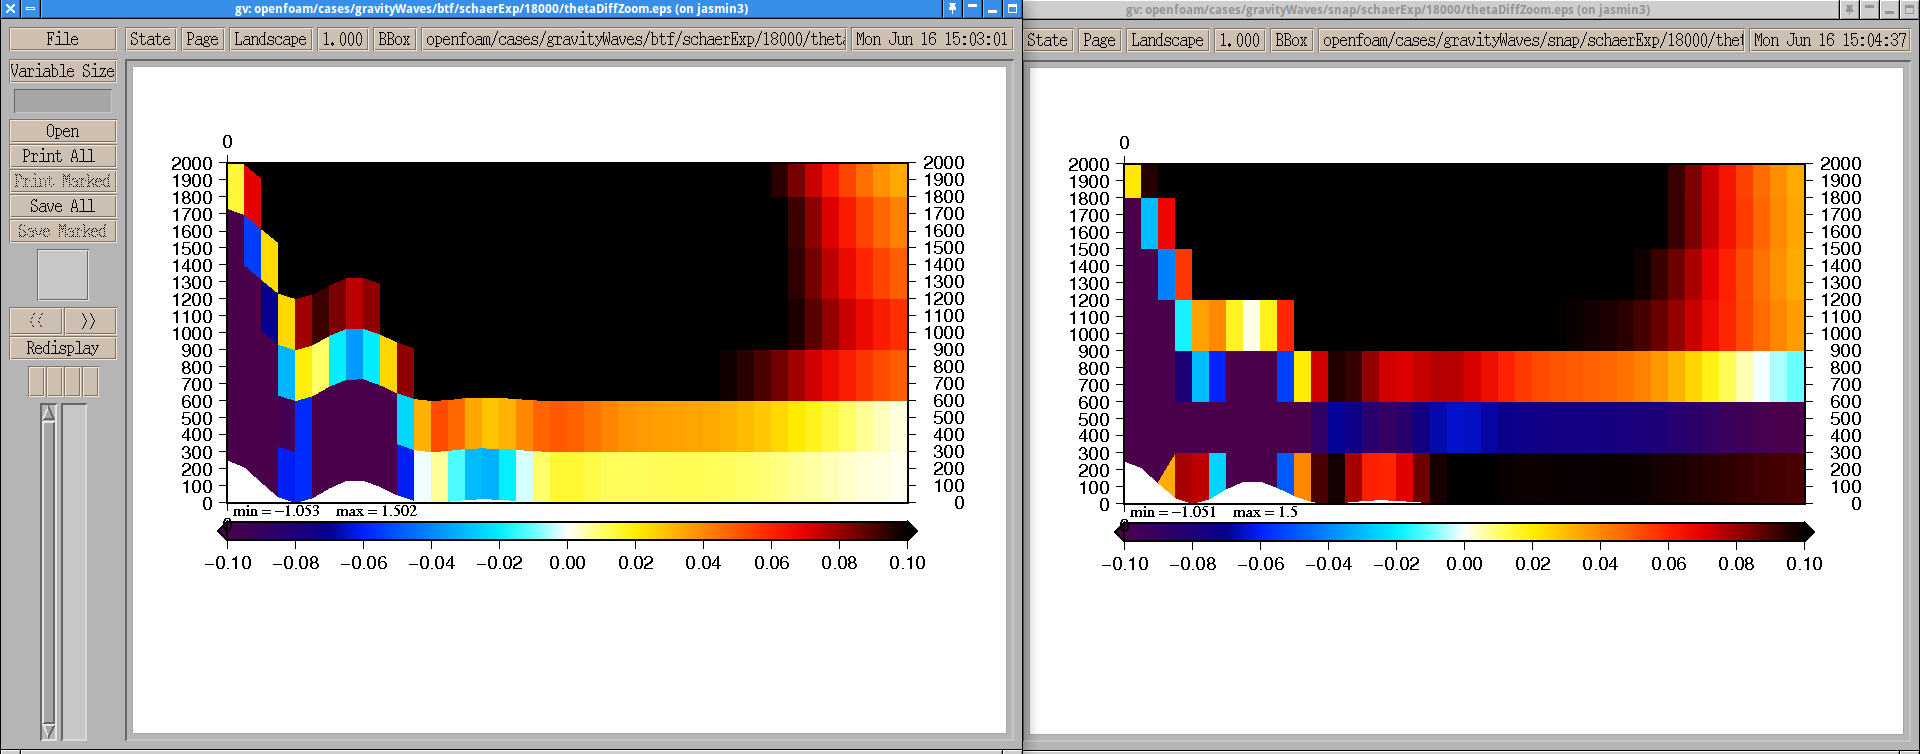
\includegraphics[width=\textwidth]{interim-results/gravityWavesBTFsnapMidZoom18000.png}
\caption{Vertical mixing after t=18000s.  Confusingly, snap mesh right, BTF left!}
\label{fig:gw:mixing-18000s}
\end{figure}

This suggests irreversible thermodynamic mixing (caused by numerical errors).  In reality, viscous effects would cause such mixing, but our equation set has no viscosity so there should be no mixing.  We can further investigate this mixing by
\begin{itemize}
	\item plotting energy changes
	\item comparing with snap/snapOrtho mesh (which have no small cells) -- TODO: which one should we use, the more orthogonal one?
	\item isolating value of nonlinear momentum term
	\item comparing with high resolution solution
\end{itemize}

\subsection{Courant number}
\begin{align}
	\mathrm{Co} = \frac{\Delta t u \cdot S}{V}
\end{align}

\begin{itemize}
	\item Mean Courant numbers for cut-cell meshes and SLEVE are lower than BTF.  This could be because cells are relatively smaller aloft.
	\item Surprisingly, mean Courant number is slightly higher for snap mesh which has no small cells (Figure~\ref{fig:gw:courant}).
	\item SLEVE and BTF have the lowest max Co numbers, snap mesh significantly higher.  Since snap mesh does not have small cells, does this imply that snap mesh has higher winds?
\end{itemize}

\begin{figure}
	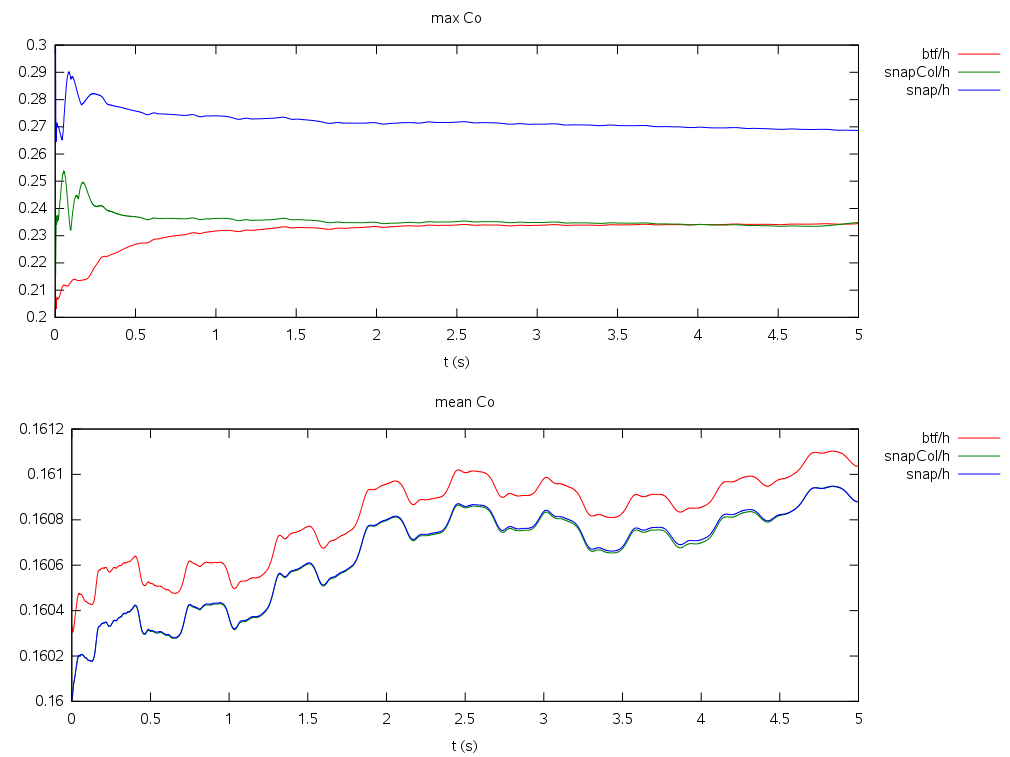
\includegraphics[width=\textwidth]{interim-results/gravityWavesCourants.png}
	\caption{Courant number for gravityWaves}
	\label{fig:gw:courant}
\end{figure}

\subsection{Energy}
\begin{itemize}
	\item Cut cell meshes are worse than TF meshes.  Snap loses internal energy much quicker than other meshes; i.e. it gets colder. (Figure~\ref{fig:gw:energy})
\end{itemize}

\begin{figure}
	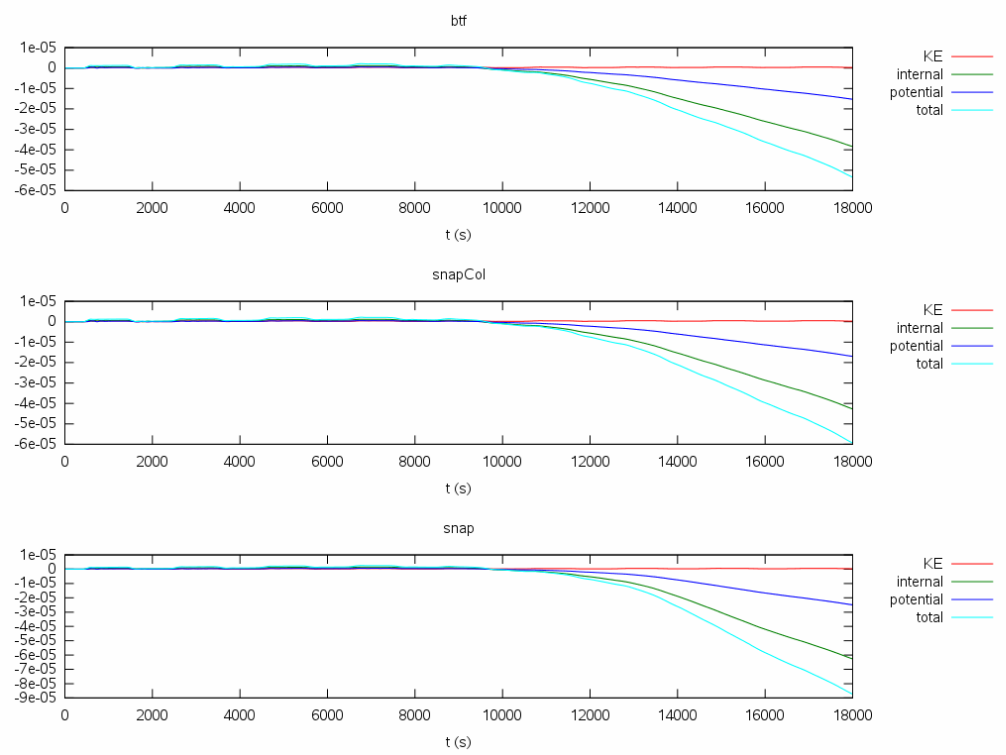
\includegraphics[width=\textwidth]{interim-results/gravityWavesEnergy.png}
	\caption{Energy changes}
	\label{fig:gw:energy}
\end{figure}

Looking at max Courant number for SLEVE, and energy loss graphs for all meshes, we see a change of behaviour at t=10000s (about 2.8 hours).  This might be related to gravity waves reflecting off the inlet or outlet boundary.  Changing the wind speed would let us investigate further.
